% ----------------------------------------------------------
% Apêndices
% ----------------------------------------------------------

% ---
% % Inicia os apêndices
% % ---
\begin{apendicesenv}

% % Imprime uma página indicando o início dos apêndices
\partapendices

\chapter{Tabela de dados}


 \label{tab:daypack}
    \begin{tabularx}{\textwidth}{p{.3\textwidth}X}
    \caption{Tabela de campos utilizados para a analise do banco de dados Loan Club}\\
    \toprule
    \textbf{Coluna} & \textbf{Descrição} \\[6pt]
    \midrule
    \endhead

annual\textunderscore inc & Renda anual relatada pelo devedor durante o cadastro.\\
delinq\textunderscore 2yrs & Incidências de inadimplência (considerados períodos de 30 dias) dentro de um período de 2 anos\\
dti\textunderscore joint & A ratio calculated using the co-borrowers' total monthly payments on the total debt obligations, excluding mortgages and the requested LC loan, divided by the co-borrowers' combined self-reported monthly income\\
earliest\textunderscore cr\textunderscore line & The month the borrower's earliest reported credit line was opened\\
emp\textunderscore length & Período em que o devedor está empregado no trabalho atual, na qual 0 representa menos de 1 ano e 10 pode ser de 10 a mais anos \\
emp\textunderscore title & Descrição breve do emprego do devedor\\
fico\textunderscore range\textunderscore high & Limite superior do score proveniente do FICO a qual o devedor está enquadrado\\
fico\textunderscore range\textunderscore low & Limite inferior do score proveniente do FICO a qual o devedor está enquadrado\\
funded\textunderscore amnt & Total do montante comprometido para aquele empréstimo até este momento\\
funded\textunderscore amnt\textunderscore inv & Total do montante comprometido pelos investidores para aquele empréstimo até este momento\\
grade & Nota atribuída pelo Loan Club\\
home\textunderscore ownership & Indica o status do tipo de moradia do tomador de empréstimo RENT (aluguel), OWN (casa própria), MORTGAGE (hipoteca), OTHER (outros)\\
id & variável de identificação de cada cliente da Loan Club\\
initial\textunderscore list\textunderscore status & The initial listing status of the loan. Possible values are – W, F\\
inq\textunderscore last\textunderscore 6mths & Quantidade de pedidos de empréstimos (excluindo carros e hipotecas)\\
installment & Pagamento devido pelo tomador de empréstimo\\
int\textunderscore rate & Taxa de juros do empréstimo\\
is\textunderscore inc\textunderscore v & Indica se a renda foi verificada pela Loan Club ou não ou se a fonte de renda foi verificada\\
issue\textunderscore d & Mês no qual o empréstimo foi financiado\\
last\textunderscore credit\textunderscore pull\textunderscore d & The most recent month LC pulled credit for this loan\\
last\textunderscore fico\textunderscore range\textunderscore high & The upper boundary range the borrower’s last FICO pulled belongs to.\\
last\textunderscore fico\textunderscore range\textunderscore low & The lower boundary range the borrower’s last FICO pulled belongs to.\\
last\textunderscore pymnt\textunderscore amnt & Valor total de pagamento recebido\\
last\textunderscore pymnt\textunderscore d & Último mês em que foi recebido um pagamento\\
loan\textunderscore amnt & The listed amount of the loan applied for by the borrower. If at some point in time, the credit department reduces the loan amount, then it will be reflected in this value.\\
loan\textunderscore status & Status atual do pagamento\\
mths\textunderscore since\textunderscore last\textunderscore delinq & Número de meses desde a última inadimplência do tomador de empréstimo\\
mths\textunderscore since\textunderscore last\textunderscore major\textunderscore derog & Months since most recent 90-day or worse rating\\
mths\textunderscore since\textunderscore last\textunderscore record & The number of months since the last public record.\\
next\textunderscore pymnt\textunderscore d & Data do próximo pagamento\\
open\textunderscore acc & Número de linhas de créditos abertas para o tomador de empréstimos\\
out\textunderscore prncp & Saldo devedor\\
out\textunderscore prncp\textunderscore inv & Remaining outstanding principal for portion of total amount funded by investors\\
policy\textunderscore code & publicly available policy\textunderscore code=1 new products not publicly available policy\textunderscore code=2\\
pub\textunderscore rec & Number of derogatory public records\\
purpose & A category provided by the borrower for the loan request. \\
pymnt\textunderscore plan & Indicates if a payment plan has been put in place for the loan\\
recoveries & post charge off gross recovery\\
revol\textunderscore bal & Total credit revolving balance\\
revol\textunderscore util & Revolving line utilization rate, or the amount of credit the borrower is using relative to all available revolving credit.\\
sub\textunderscore grade & LC assigned loan subgrade\\
term & Quantidade de pagamentos do empréstimos que pode ser de 36 ou 60 meses\\
title & Tipo de empréstimo realizado pelo mutuário\\
total\textunderscore acc & The total number of credit lines currently in the borrower's credit file\\
total\textunderscore pymnt & Pagamentos recebidos até o momento presente sobre o valor financiado\\
total\textunderscore pymnt\textunderscore inv & Pagamentos recebidos até o momento presente sobre o valor financiado pelo investidor\\
total\textunderscore rec\textunderscore int & Juros recebido até a data presente\\
total\textunderscore rec\textunderscore late\textunderscore fee & Taxas de atraso recebido até a presente data\\
total\textunderscore rec\textunderscore prncp & Principal received to date\\
verified\textunderscore status\textunderscore joint & Indicates if the co-borrowers' joint income was verified by LC, not verified, or if the income source was verified\\
zip\textunderscore code & Os primeiros 3 números de código postal fornecida pelo tomador de empréstimo\\
open\textunderscore acc\textunderscore 6m & Number of open trades in last 6 months\\
open\textunderscore il\textunderscore 6m & Number of currently active installment trades\\
open\textunderscore il\textunderscore 12m & Number of installment accounts opened in past 12 months\\
open\textunderscore il\textunderscore 24m & Number of installment accounts opened in past 24 months\\
mths\textunderscore since\textunderscore rcnt\textunderscore il & Months since most recent installment accounts opened\\
total\textunderscore bal\textunderscore il & Total current balance of all installment accounts\\
il\textunderscore util & Ratio of total current balance to high credit/credit limit on all install acct\\
open\textunderscore rv\textunderscore 12m & Number of revolving trades opened in past 12 months\\
open\textunderscore rv\textunderscore 24m & Number of revolving trades opened in past 24 months\\
max\textunderscore bal\textunderscore bc & Maximum current balance owed on all revolving accounts\\
all\textunderscore util & Balance to credit limit on all trades\\
total\textunderscore rev\textunderscore hi\textunderscore lim & Total revolving high credit/credit limit\\
inq\textunderscore fi & Number of personal finance inquiries\\
total\textunderscore cu\textunderscore tl & Número de negócios financeiros\\
inq\textunderscore last\textunderscore 12m & Number of credit inquiries in past 12 months\\
acc\textunderscore now\textunderscore delinq & Número de contas nas quais o mutuário está agora inadimplente\\
tot\textunderscore coll\textunderscore amt & Total collection amounts ever owed \\
tot\textunderscore cur\textunderscore bal & Total current balance of all accounts \\

\bottomrule

\end{tabularx}


 \label{tab:daypack}
    \begin{tabularx}{\textwidth}{p{.3\textwidth}X}
    \caption{Tabela de campos disponíveis em Loan Club}\\
    \toprule
    \textbf{Coluna} & \textbf{Descrição} \\[6pt]
    \midrule
    \endhead

addr\textunderscore state & The state provided by the borrower in the loan application\\
annual\textunderscore inc & The self-reported annual income provided by the borrower during registration.\\
annual\textunderscore inc\textunderscore joint & The combined self-reported annual income provided by the co-borrowers during registration\\
application\textunderscore type & Indicates whether the loan is an individual application or a joint application with two co-borrowers\\
collection\textunderscore recovery\textunderscore fee & post charge off collection fee\\
collections\textunderscore 12\textunderscore mths\textunderscore ex\textunderscore med & Number of collections in 12 months excluding medical collections\\
delinq\textunderscore 2yrs & The number of 30+ days past-due incidences of delinquency in the borrower's credit file for the past 2 years\\
desc & Loan description provided by the borrower\\
dti & A ratio calculated using the borrower’s total monthly debt payments on the total debt obligations, excluding mortgage and the requested LC loan, divided by the borrower’s self-reported monthly income.\\
dti\textunderscore joint & A ratio calculated using the co-borrowers' total monthly payments on the total debt obligations, excluding mortgages and the requested LC loan, divided by the co-borrowers' combined self-reported monthly income\\
earliest\textunderscore cr\textunderscore line & The month the borrower's earliest reported credit line was opened\\
emp\textunderscore length & Employment length in years. Possible values are between 0 and 10 where 0 means less than one year and 10 means ten or more years. \\
emp\textunderscore title & The job title supplied by the Borrower when applying for the loan.*\\
fico\textunderscore range\textunderscore high & The upper boundary range the borrower’s FICO at loan origination belongs to.\\
fico\textunderscore range\textunderscore low & The lower boundary range the borrower’s FICO at loan origination belongs to.\\
funded\textunderscore amnt & The total amount committed to that loan at that point in time.\\
funded\textunderscore amnt\textunderscore inv & The total amount committed by investors for that loan at that point in time.\\
grade & LC assigned loan grade\\
home\textunderscore ownership & The home ownership status provided by the borrower during registration. Our values are: RENT, OWN, MORTGAGE, OTHER.\\
id & A unique LC assigned ID for the loan listing.\\
initial\textunderscore list\textunderscore status & The initial listing status of the loan. Possible values are – W, F\\
inq\textunderscore last\textunderscore 6mths & The number of inquiries in past 6 months (excluding auto and mortgage inquiries)\\
installment & The monthly payment owed by the borrower if the loan originates.\\
int\textunderscore rate & Interest Rate on the loan\\
is\textunderscore inc\textunderscore v & Indicates if income was verified by LC, not verified, or if the income source was verified\\
issue\textunderscore d & The month which the loan was funded\\
last\textunderscore credit\textunderscore pull\textunderscore d & The most recent month LC pulled credit for this loan\\
last\textunderscore fico\textunderscore range\textunderscore high & The upper boundary range the borrower’s last FICO pulled belongs to.\\
last\textunderscore fico\textunderscore range\textunderscore low & The lower boundary range the borrower’s last FICO pulled belongs to.\\
last\textunderscore pymnt\textunderscore amnt & Last total payment amount received\\
last\textunderscore pymnt\textunderscore d & Last month payment was received\\
loan\textunderscore amnt & The listed amount of the loan applied for by the borrower. If at some point in time, the credit department reduces the loan amount, then it will be reflected in this value.\\
loan\textunderscore status & Current status of the loan\\
member\textunderscore id & A unique LC assigned Id for the borrower member.\\
mths\textunderscore since\textunderscore last\textunderscore delinq & The number of months since the borrower's last delinquency.\\
mths\textunderscore since\textunderscore last\textunderscore major\textunderscore derog & Months since most recent 90-day or worse rating\\
mths\textunderscore since\textunderscore last\textunderscore record & The number of months since the last public record.\\
next\textunderscore pymnt\textunderscore d & Next scheduled payment date\\
open\textunderscore acc & The number of open credit lines in the borrower's credit file.\\
out\textunderscore prncp & emaining outstanding principal for total amount funded\\
out\textunderscore prncp\textunderscore inv & Remaining outstanding principal for portion of total amount funded by investors\\
policy\textunderscore code & "publicly available policy\textunderscore code=1\\
new products not publicly available policy\textunderscore code=2"\\
pub\textunderscore rec & Number of derogatory public records\\
purpose & A category provided by the borrower for the loan request. \\
pymnt\textunderscore plan & Indicates if a payment plan has been put in place for the loan\\
recoveries & post charge off gross recovery\\
revol\textunderscore bal & Total credit revolving balance\\
revol\textunderscore util & Revolving line utilization rate, or the amount of credit the borrower is using relative to all available revolving credit.\\
sub\textunderscore grade & LC assigned loan subgrade\\
term & The number of payments on the loan. Values are in months and can be either 36 or 60.\\
title & The loan title provided by the borrower\\
total\textunderscore acc & The total number of credit lines currently in the borrower's credit file\\
total\textunderscore pymnt & Payments received to date for total amount funded\\
total\textunderscore pymnt\textunderscore inv & Payments received to date for portion of total amount funded by investors\\
total\textunderscore rec\textunderscore int & Interest received to date\\
total\textunderscore rec\textunderscore late\textunderscore fee & Late fees received to date\\
total\textunderscore rec\textunderscore prncp & Principal received to date\\
verified\textunderscore status\textunderscore joint & Indicates if the co-borrowers' joint income was verified by LC, not verified, or if the income source was verified\\
zip\textunderscore code & The first 3 numbers of the zip code provided by the borrower in the loan application.\\
open\textunderscore acc\textunderscore 6m & Number of open trades in last 6 months\\
open\textunderscore il\textunderscore 6m & Number of currently active installment trades\\
open\textunderscore il\textunderscore 12m & Number of installment accounts opened in past 12 months\\
open\textunderscore il\textunderscore 24m & Number of installment accounts opened in past 24 months\\
mths\textunderscore since\textunderscore rcnt\textunderscore il & Months since most recent installment accounts opened\\
total\textunderscore bal\textunderscore il & Total current balance of all installment accounts\\
il\textunderscore util & Ratio of total current balance to high credit/credit limit on all install acct\\
open\textunderscore rv\textunderscore 12m & Number of revolving trades opened in past 12 months\\
open\textunderscore rv\textunderscore 24m & Number of revolving trades opened in past 24 months\\
max\textunderscore bal\textunderscore bc & Maximum current balance owed on all revolving accounts\\
all\textunderscore util & Balance to credit limit on all trades\\
total\textunderscore rev\textunderscore hi\textunderscore lim & Total revolving high credit/credit limit\\
inq\textunderscore fi & Number of personal finance inquiries\\
total\textunderscore cu\textunderscore tl & Number of finance trades\\
inq\textunderscore last\textunderscore 12m & Number of credit inquiries in past 12 months\\
acc\textunderscore now\textunderscore delinq & The number of accounts on which the borrower is now delinquent.\\
tot\textunderscore coll\textunderscore amt & Total collection amounts ever owed \\
tot\textunderscore cur\textunderscore bal & Total current balance of all accounts \\

\bottomrule

\end{tabularx}

\chapter{Análise dos clusters vs grades}

\begin{figure*}[t!]
    \centering
        \caption{collection\textunderscore recovery\textunderscore fee }
    	\begin{subfigure}[t]{0.5\textwidth}
    		\centering
        	\caption{Cluster }

			\centerline{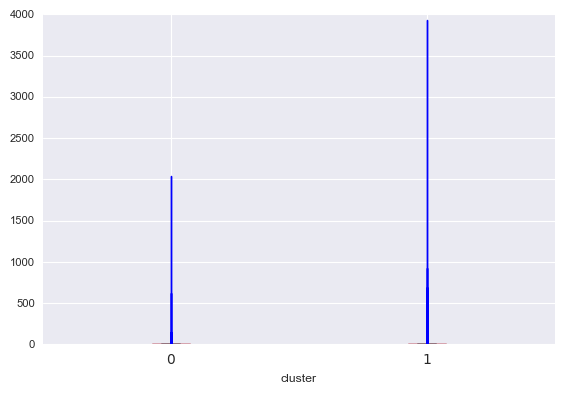
\includegraphics[width=1\textwidth]{img/collection_recovery_fee_by_cluster}}
    	\end{subfigure}%
    	~ 
    	\begin{subfigure}[t]{0.5\textwidth}
    		\centering
        	\caption{Grade }
   
			\centerline{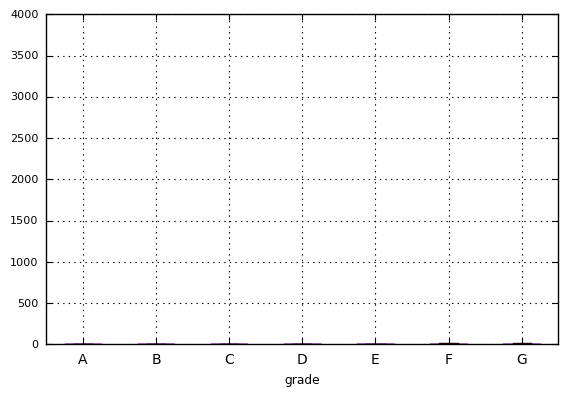
\includegraphics[width=1\textwidth]{img/collection_recovery_fee_by_grade}}

    	\end{subfigure}
    	\\
    	        \caption{funded\textunderscore amnt}
    	\begin{subfigure}[t]{0.5\textwidth}
    		\centering

			\centerline{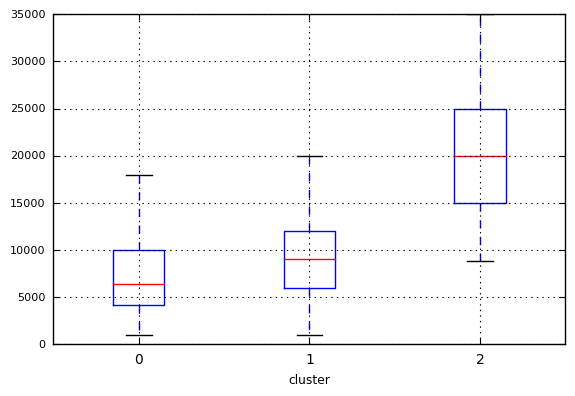
\includegraphics[width=1.05\textwidth]{img/funded_amnt_by_cluster}}
    	\end{subfigure}%
    	~ 
    	\begin{subfigure}[t]{0.5\textwidth}
    		\centering
   
			\centerline{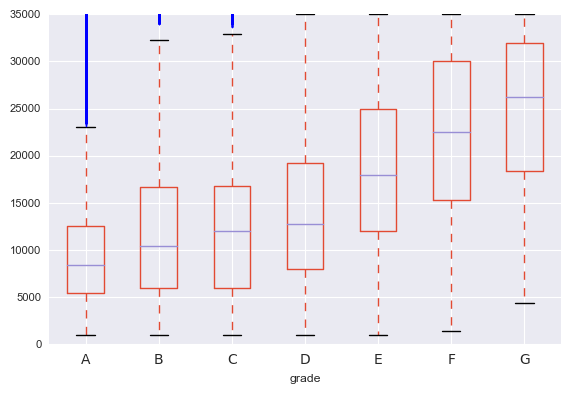
\includegraphics[width=1.05\textwidth]{img/funded_amnt_by_grade}}

    	\end{subfigure}

\end{figure*}

\begin{figure*}[t!]
    \centering
        \caption{funded\textunderscore amnt\textunderscore inv }
    	\begin{subfigure}[t]{0.5\textwidth}
 
			\centerline{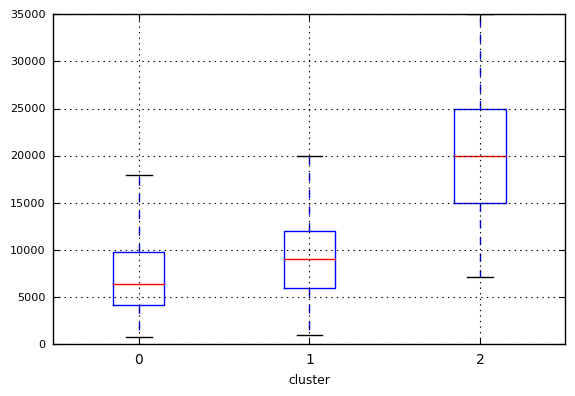
\includegraphics[width=1\textwidth]{img/funded_amnt_inv_by_cluster}}
    	\end{subfigure}%
    	~ 
    	\begin{subfigure}[t]{0.5\textwidth}
 			\centerline{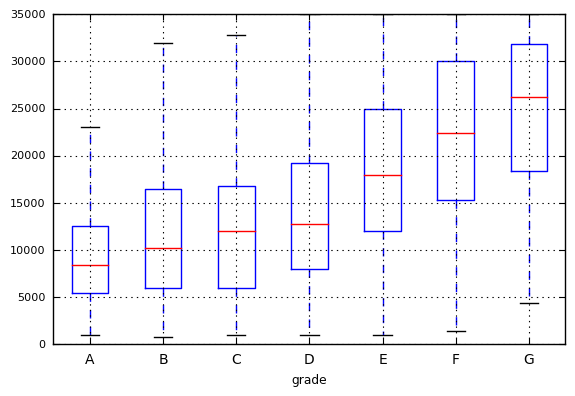
\includegraphics[width=1\textwidth]{img/funded_amnt_inv_by_grade}}

    	\end{subfigure}
    	\\
    	        \caption{installment}
    	\begin{subfigure}[t]{0.5\textwidth}
    		\centering

			\centerline{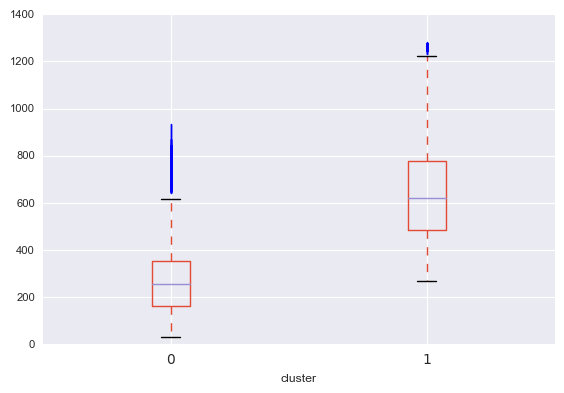
\includegraphics[width=1.05\textwidth]{img/installment_by_cluster}}
    	\end{subfigure}%
    	~ 
    	\begin{subfigure}[t]{0.5\textwidth}
    		\centering
   
			\centerline{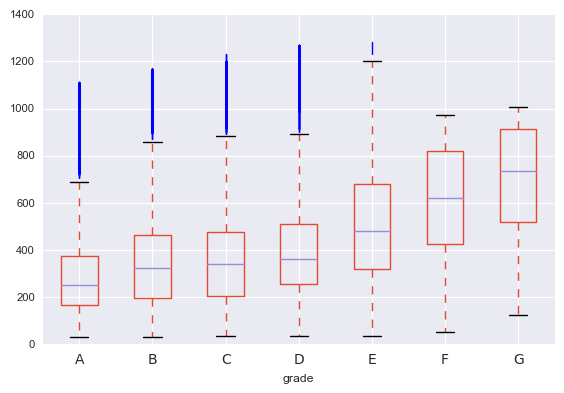
\includegraphics[width=1.05\textwidth]{img/installment_by_grade}}

    	\end{subfigure}



\end{figure*}

\begin{figure*}[t!]
    \centering
        \caption{term\textunderscore float\textunderscore fee }
    	\begin{subfigure}[t]{0.5\textwidth}
    		\centering

			\centerline{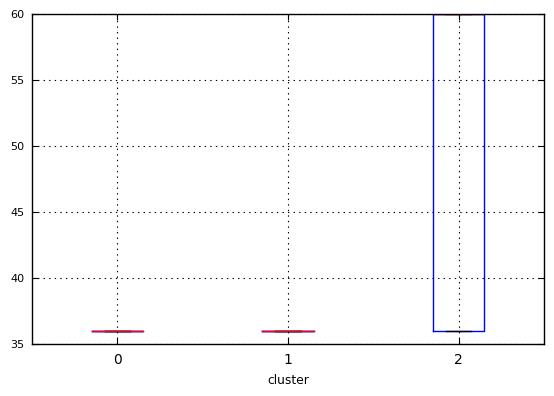
\includegraphics[width=1\textwidth]{img/term_float_by_cluster}}
    	\end{subfigure}%
    	~ 
    	\begin{subfigure}[t]{0.5\textwidth}
    		\centering
   
			\centerline{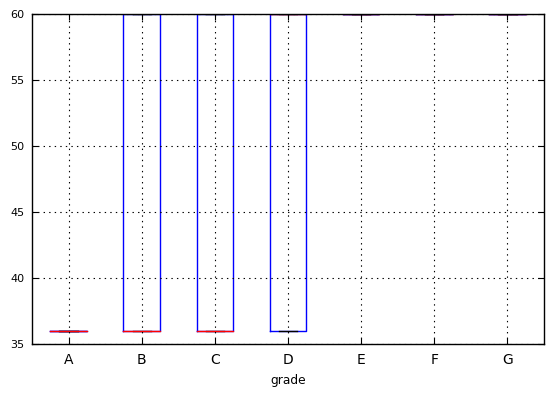
\includegraphics[width=1\textwidth]{img/term_float_by_grade}}

    	\end{subfigure}
    	\\
    	        \caption{loan\textunderscore amnt}
    	\begin{subfigure}[t]{0.5\textwidth}
    		\centering

			\centerline{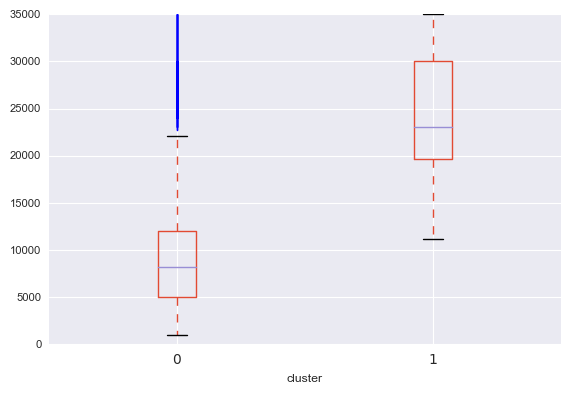
\includegraphics[width=1.05\textwidth]{img/loan_amnt_by_cluster}}
    	\end{subfigure}%
    	~ 
    	\begin{subfigure}[t]{0.5\textwidth}
    		\centering
   
			\centerline{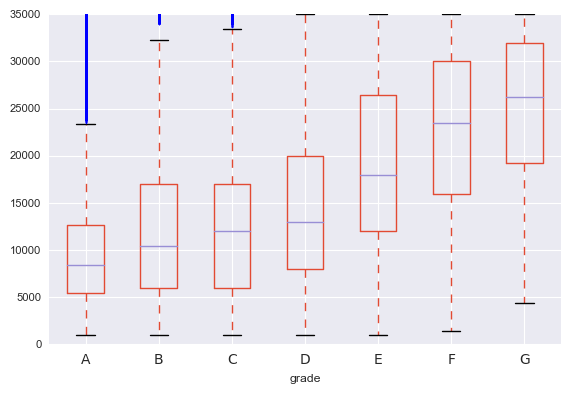
\includegraphics[width=1.05\textwidth]{img/loan_amnt_by_grade}}

    	\end{subfigure}
\\
    	        \caption{int\textunderscore rate\textunderscore float}
    	\begin{subfigure}[t]{0.5\textwidth}
    		\centering

			\centerline{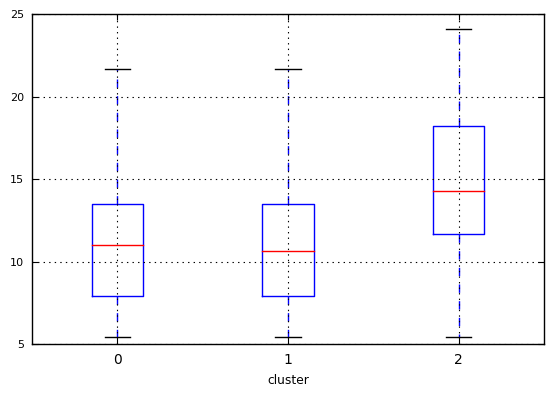
\includegraphics[width=1.05\textwidth]{img/int_rate_float_by_cluster}}
    	\end{subfigure}%
    	~ 
    	\begin{subfigure}[t]{0.5\textwidth}
    		\centering
   
			\centerline{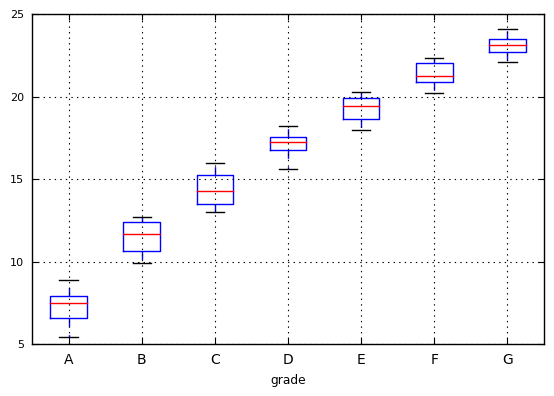
\includegraphics[width=1.05\textwidth]{img/int_rate_float_by_grade}}

    	\end{subfigure}
\end{figure*}



\begin{figure*}[t!]
    \centering
        \caption{annual\textunderscore inc }
    	\begin{subfigure}[t]{0.5\textwidth}
    		\centering

			\centerline{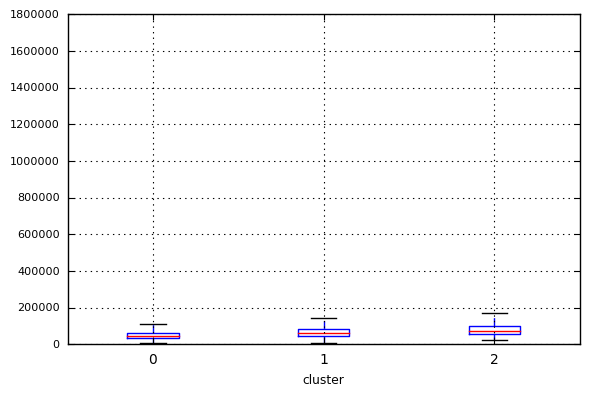
\includegraphics[width=1\textwidth]{img/annual_inc_by_cluster}}
    	\end{subfigure}%
    	~ 
    	\begin{subfigure}[t]{0.5\textwidth}
    		\centering
   
			\centerline{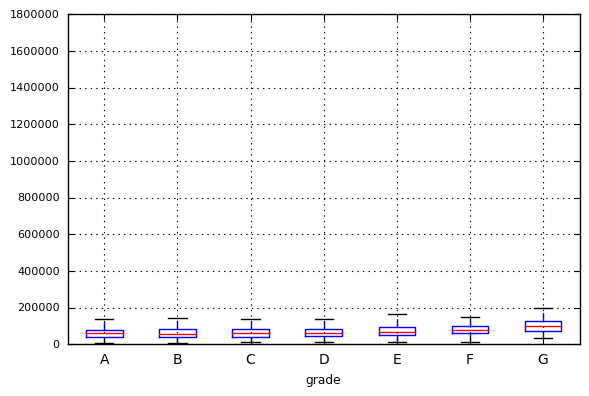
\includegraphics[width=1\textwidth]{img/annual_inc_by_grade}}

    	\end{subfigure}
    	\\
    	        \caption{delinq\textunderscore 2yrs}
    	\begin{subfigure}[t]{0.5\textwidth}
    		\centering

			\centerline{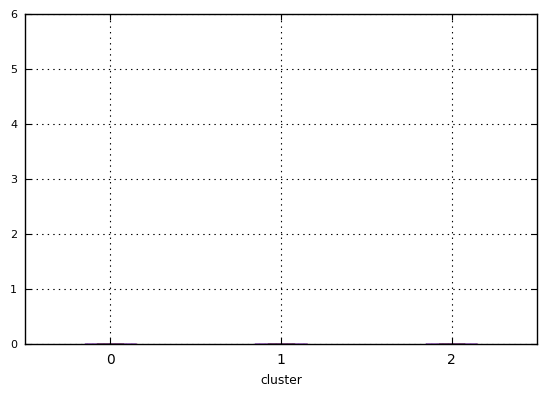
\includegraphics[width=1.05\textwidth]{img/delinq_2yrs_by_cluster}}
    	\end{subfigure}%
    	~ 
    	\begin{subfigure}[t]{0.5\textwidth}
    		\centering
   
			\centerline{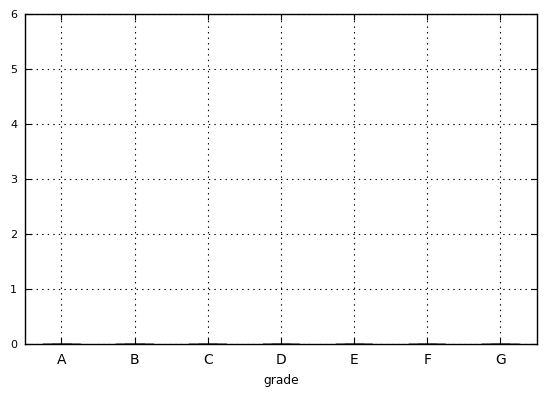
\includegraphics[width=1.05\textwidth]{img/delinq_2yrs_by_grade}}

    	\end{subfigure}
\\
    	        \caption{recoveries}
    	\begin{subfigure}[t]{0.5\textwidth}
    		\centering

			\centerline{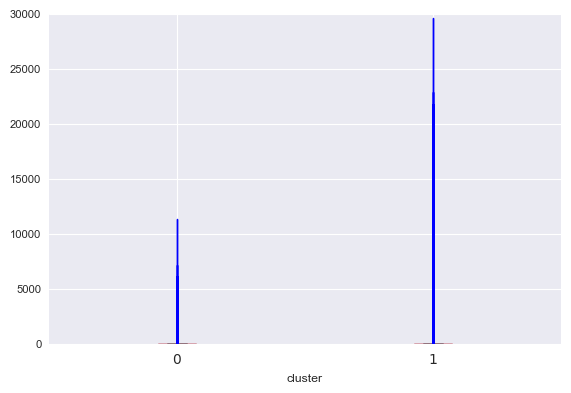
\includegraphics[width=1.05\textwidth]{img/recoveries_by_cluster}}
    	\end{subfigure}%
    	~ 
    	\begin{subfigure}[t]{0.5\textwidth}
    		\centering
   
			\centerline{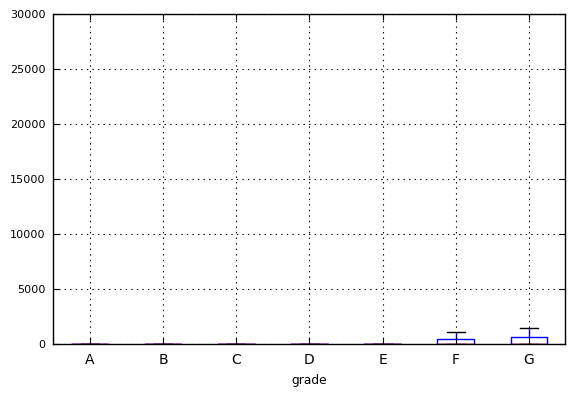
\includegraphics[width=1.05\textwidth]{img/recoveries_by_grade}}

    	\end{subfigure}
\end{figure*}


\begin{figure*}[t!]
    \centering
        \caption{open\textunderscore acc }
    	\begin{subfigure}[t]{0.5\textwidth}
    		\centering

			\centerline{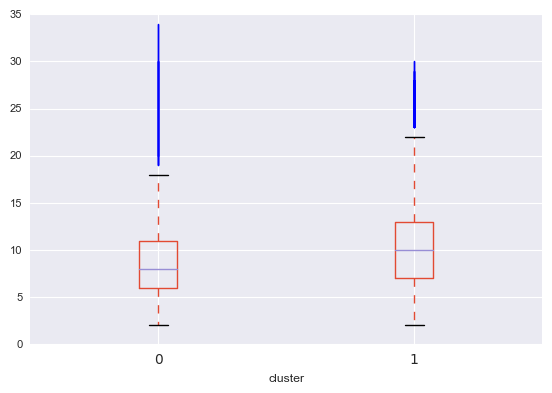
\includegraphics[width=1\textwidth]{img/open_acc_by_cluster}}
    	\end{subfigure}%
    	~ 
    	\begin{subfigure}[t]{0.5\textwidth}
    		\centering
   
			\centerline{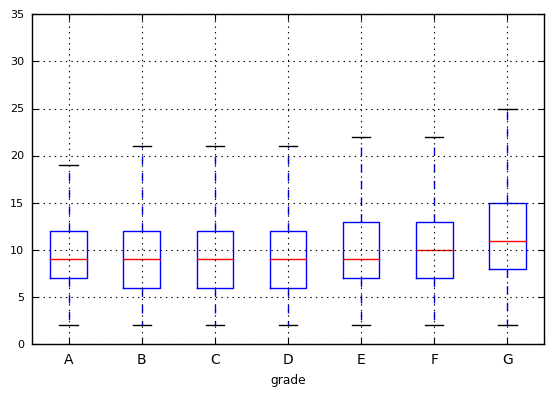
\includegraphics[width=1\textwidth]{img/open_acc_by_grade}}

    	\end{subfigure}
    	\\
    	        \caption{pub\textunderscore rec}
    	\begin{subfigure}[t]{0.5\textwidth}
    		\centering

			\centerline{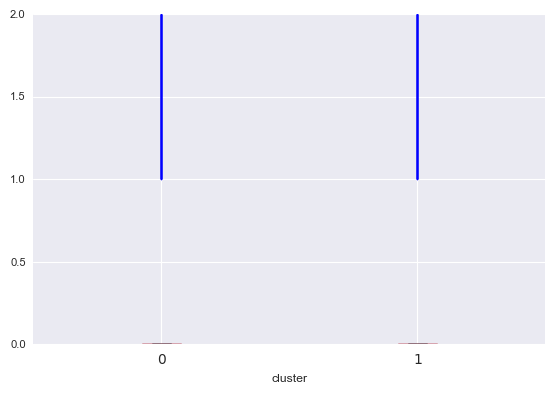
\includegraphics[width=1.05\textwidth]{img/pub_rec_by_cluster}}
    	\end{subfigure}%
    	~ 
    	\begin{subfigure}[t]{0.5\textwidth}
    		\centering
   
			\centerline{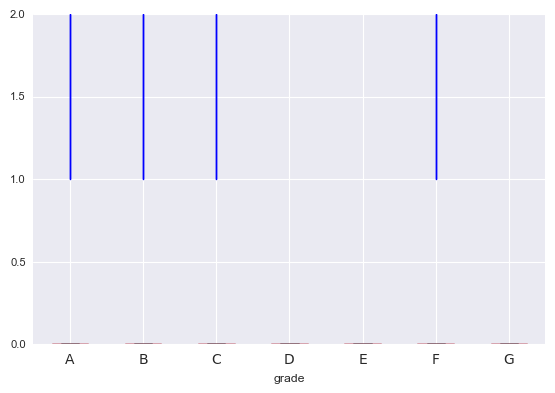
\includegraphics[width=1.05\textwidth]{img/pub_rec_by_grade}}

    	\end{subfigure}
\\
    	        \caption{inq\textunderscore last\textunderscore 6mths}
    	\begin{subfigure}[t]{0.5\textwidth}
    		\centering

			\centerline{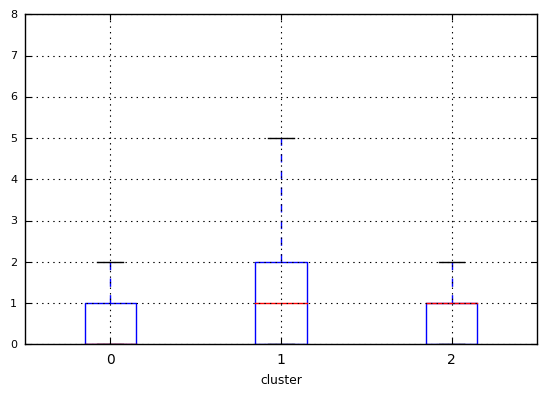
\includegraphics[width=1.05\textwidth]{img/inq_last_6mths_by_cluster}}
    	\end{subfigure}%
    	~ 
    	\begin{subfigure}[t]{0.5\textwidth}
    		\centering
   
			\centerline{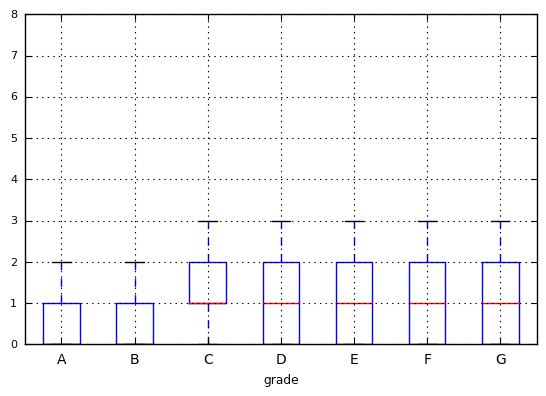
\includegraphics[width=1.05\textwidth]{img/inq_last_6mths_by_grade}}

    	\end{subfigure}
\end{figure*}

\begin{figure*}[t!]
    \centering
        \caption{revol\textunderscore bal }
    	\begin{subfigure}[t]{0.5\textwidth}
    		\centering

			\centerline{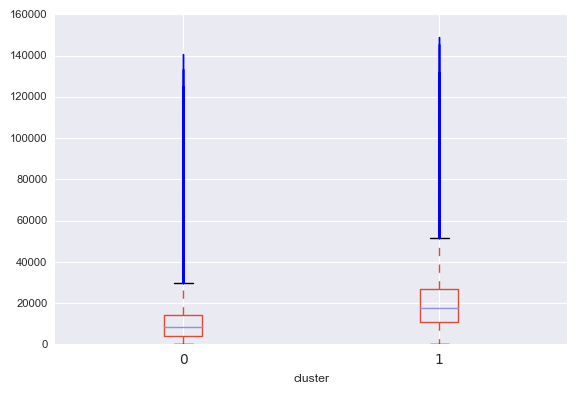
\includegraphics[width=1\textwidth]{img/revol_bal_by_cluster}}
    	\end{subfigure}%
    	~ 
    	\begin{subfigure}[t]{0.5\textwidth}
    		\centering
   
			\centerline{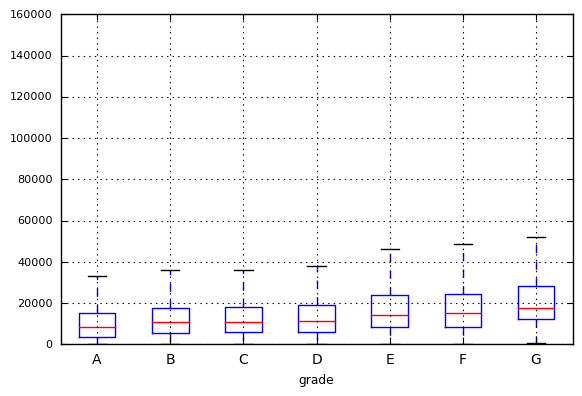
\includegraphics[width=1\textwidth]{img/revol_bal_by_grade}}

    	\end{subfigure}
    	\\
    	        \caption{total\textunderscore acc}
    	\begin{subfigure}[t]{0.5\textwidth}
    		\centering

			\centerline{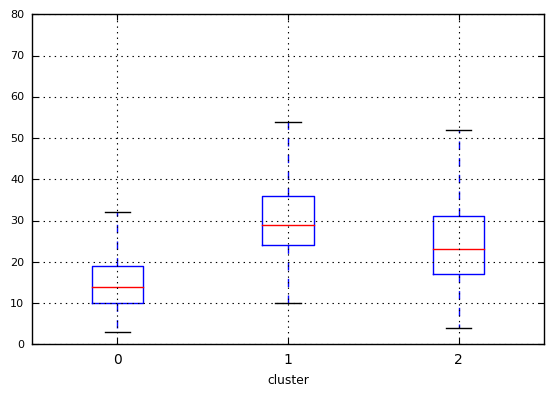
\includegraphics[width=1.05\textwidth]{img/total_acc_by_cluster}}
    	\end{subfigure}%
    	~ 
    	\begin{subfigure}[t]{0.5\textwidth}
    		\centering
   
			\centerline{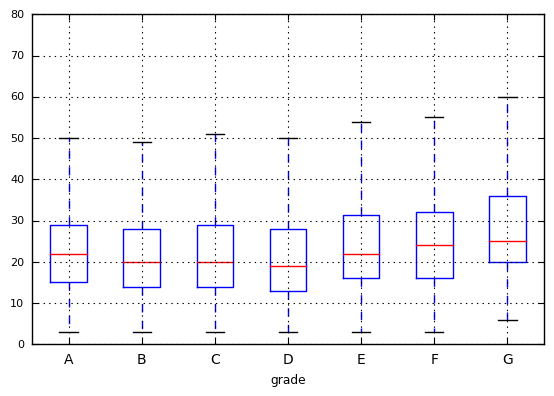
\includegraphics[width=1.05\textwidth]{img/total_acc_by_grade}}

    	\end{subfigure}
\\
    	        \caption{out\textunderscore prncp}
    	\begin{subfigure}[t]{0.5\textwidth}
    		\centering

			\centerline{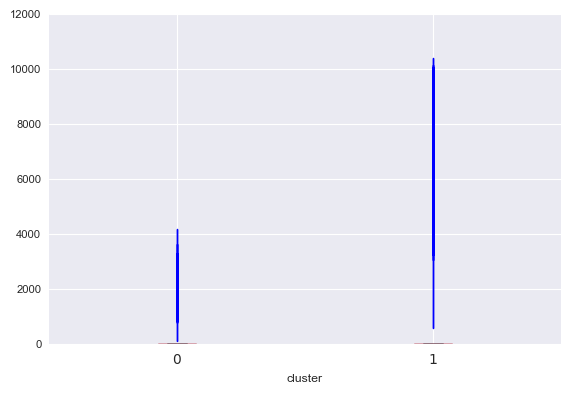
\includegraphics[width=1.05\textwidth]{img/out_prncp_by_cluster}}
    	\end{subfigure}%
    	~ 
    	\begin{subfigure}[t]{0.5\textwidth}
    		\centering
   
			\centerline{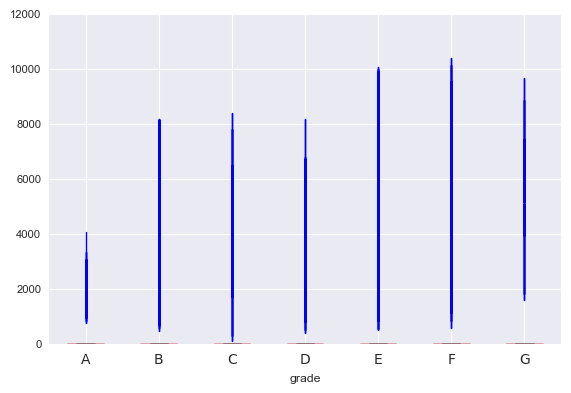
\includegraphics[width=1.05\textwidth]{img/out_prncp_by_grade}}

    	\end{subfigure}
\end{figure*}


\begin{figure*}[t!]
    \centering
        \caption{total\textunderscore pymnt }
    	\begin{subfigure}[t]{0.5\textwidth}
    		\centering

			\centerline{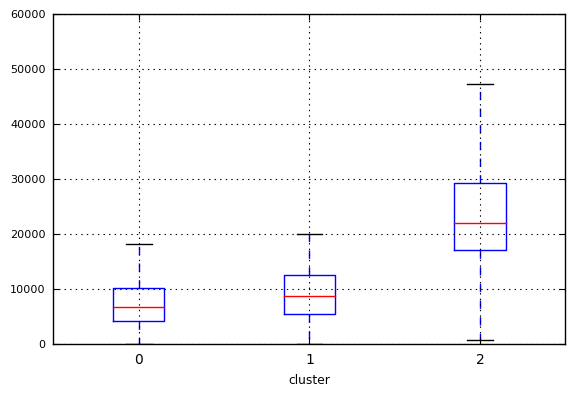
\includegraphics[width=1\textwidth]{img/total_pymnt_by_cluster}}
    	\end{subfigure}%
    	~ 
    	\begin{subfigure}[t]{0.5\textwidth}
    		\centering
   
			\centerline{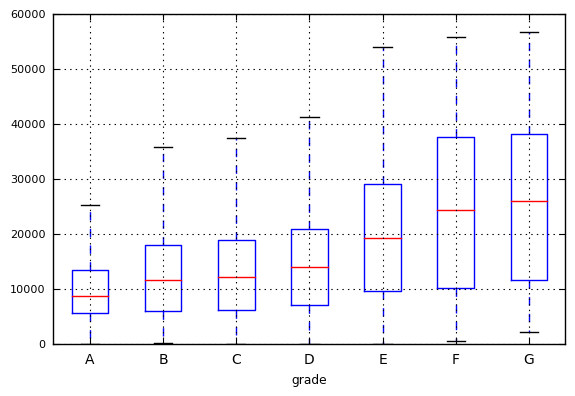
\includegraphics[width=1\textwidth]{img/total_pymnt_by_grade}}

    	\end{subfigure}
    	\\
    	        \caption{out\textunderscore prncp\textunderscore inv}
    	\begin{subfigure}[t]{0.5\textwidth}
    		\centering

			\centerline{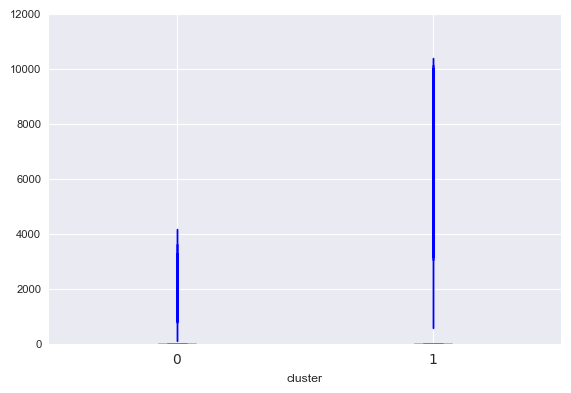
\includegraphics[width=1.05\textwidth]{img/out_prncp_inv_by_cluster}}
    	\end{subfigure}%
    	~ 
    	\begin{subfigure}[t]{0.5\textwidth}
    		\centering
   
			\centerline{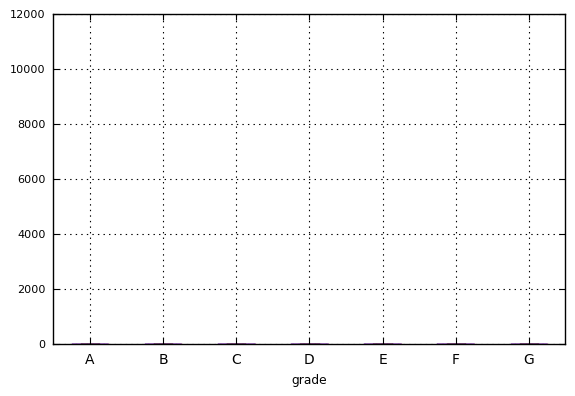
\includegraphics[width=1.05\textwidth]{img/out_prncp_inv_by_grade}}

    	\end{subfigure}
\\
    	        \caption{total\textunderscore rec\textunderscore int }
    	\begin{subfigure}[t]{0.5\textwidth}
    		\centering

			\centerline{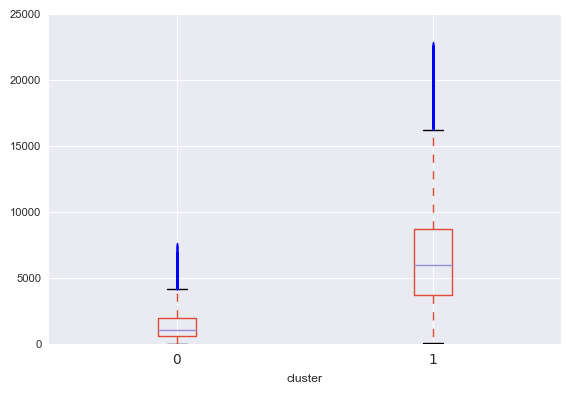
\includegraphics[width=1.05\textwidth]{img/total_rec_int_by_cluster}}
    	\end{subfigure}%
    	~ 
    	\begin{subfigure}[t]{0.5\textwidth}
    		\centering
   
			\centerline{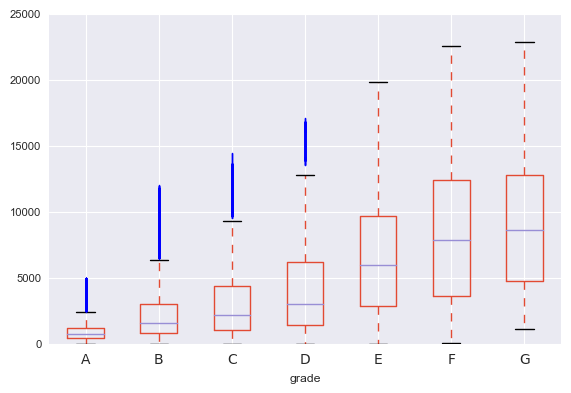
\includegraphics[width=1.05\textwidth]{img/total_rec_int_by_grade}}

    	\end{subfigure}
\end{figure*}



\begin{figure*}[t!]
    \centering
        \caption{total\textunderscore pymnt\textunderscore inv }
    	\begin{subfigure}[t]{0.5\textwidth}
    		\centering

			\centerline{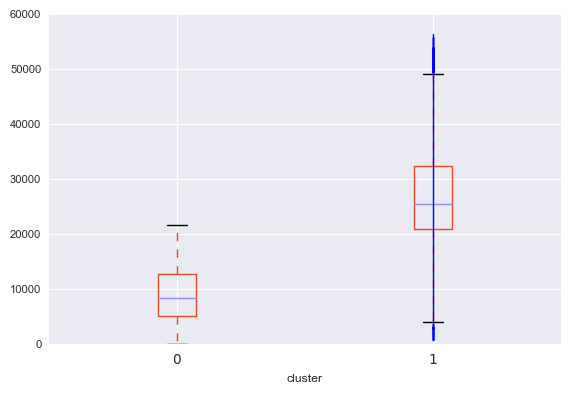
\includegraphics[width=1\textwidth]{img/total_pymnt_inv_by_cluster}}
    	\end{subfigure}%
    	~ 
    	\begin{subfigure}[t]{0.5\textwidth}
    		\centering
   
			\centerline{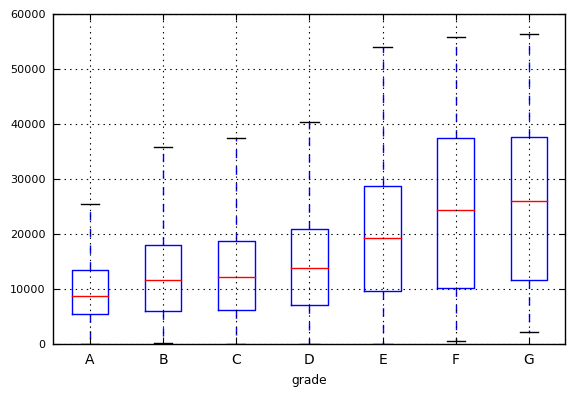
\includegraphics[width=1\textwidth]{img/total_pymnt_inv_by_grade}}

    	\end{subfigure}
    	\\
    	        \caption{last\textunderscore pymnt\textunderscore amnt}
    	\begin{subfigure}[t]{0.5\textwidth}
    		\centering

			\centerline{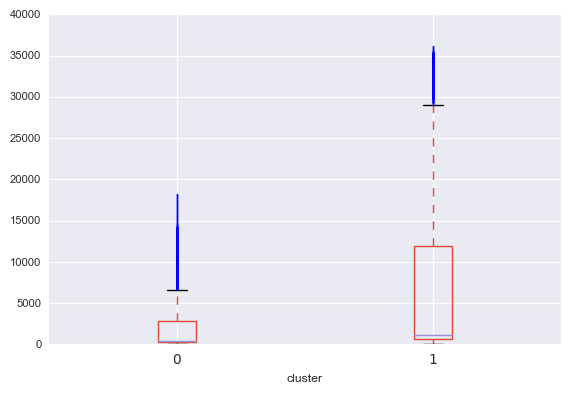
\includegraphics[width=1.05\textwidth]{img/last_pymnt_amnt_by_cluster}}
    	\end{subfigure}%
    	~ 
    	\begin{subfigure}[t]{0.5\textwidth}
    		\centering
   
			\centerline{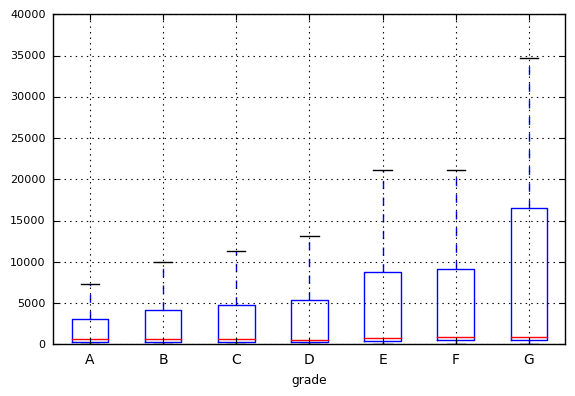
\includegraphics[width=1.05\textwidth]{img/last_pymnt_amnt_by_grade}}

    	\end{subfigure}
\\
    	        \caption{total\textunderscore rec\textunderscore prncp }
    	\begin{subfigure}[t]{0.5\textwidth}
    		\centering

			\centerline{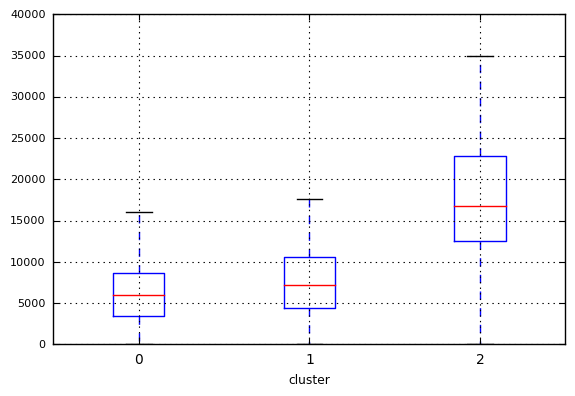
\includegraphics[width=1.05\textwidth]{img/total_rec_prncp_by_cluster}}
    	\end{subfigure}%
    	~ 
    	\begin{subfigure}[t]{0.5\textwidth}
    		\centering
   
			\centerline{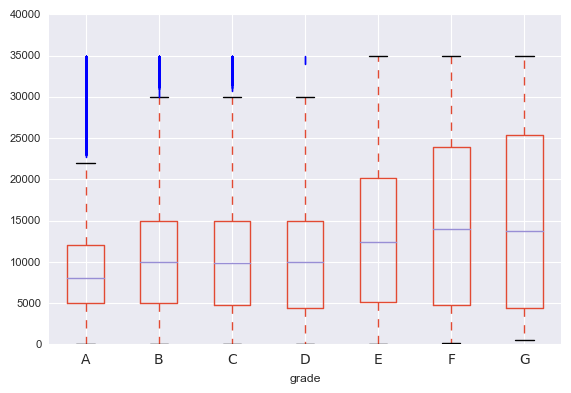
\includegraphics[width=1.05\textwidth]{img/total_rec_prncp_by_grade}}

    	\end{subfigure}
\end{figure*}



\begin{figure*}[t!]
    \centering
        \caption{total\textunderscore rec\textunderscore late\textunderscore fee }
    	\begin{subfigure}[t]{0.5\textwidth}
    		\centering

			\centerline{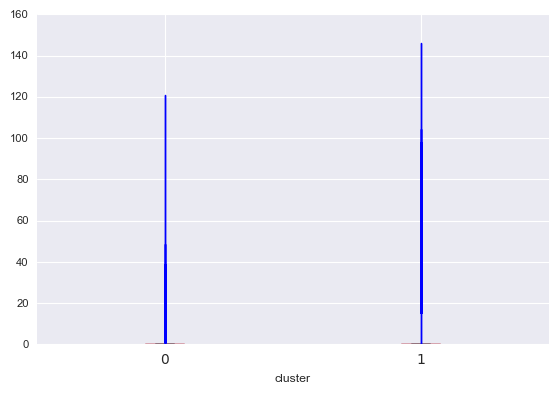
\includegraphics[width=1\textwidth]{img/total_rec_late_fee_by_cluster}}
    	\end{subfigure}%
    	~ 
    	\begin{subfigure}[t]{0.5\textwidth}
    		\centering
   
			\centerline{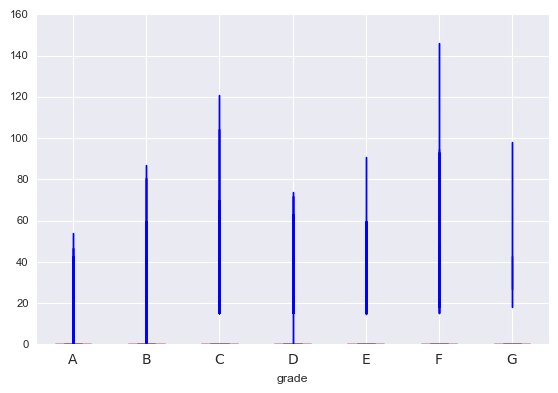
\includegraphics[width=1\textwidth]{img/total_rec_late_fee_by_grade}}

    	\end{subfigure}
    	    	\\
    	        \caption{dti}
    	\begin{subfigure}[t]{0.5\textwidth}
    		\centering

			\centerline{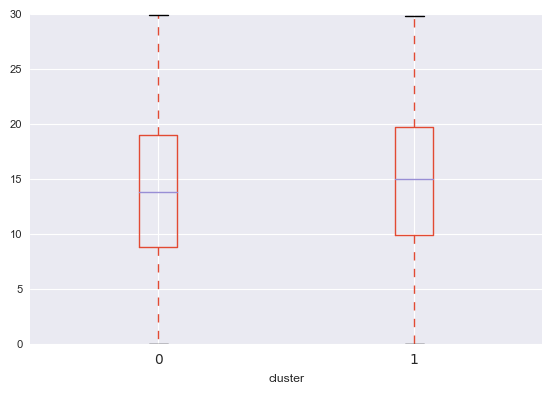
\includegraphics[width=1.05\textwidth]{img/dti_by_cluster}}
    	\end{subfigure}%
    	~ 
    	\begin{subfigure}[t]{0.5\textwidth}
    		\centering
   
			\centerline{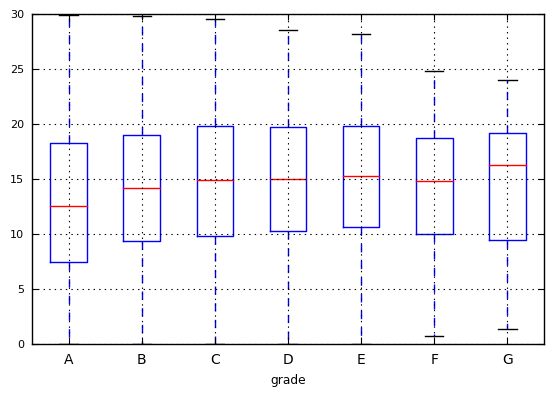
\includegraphics[width=1.05\textwidth]{img/dti_by_grade}}

    	\end{subfigure}
\end{figure*}



\chapter{Correlacao entre variaveis}


\begin{landscape}

\begin{table}[]
\centering
\caption{My caption}
\label{my-label}


\begin{tabular}{lrrrrrrrrrrrrrrrrrrrrrrrrr}
                          & funded\_amnt & funded\_amnt\_inv & loan\_amnt & term\_float & int\_rate\_float & installment & annual\_inc & dti     & delinq\_2yrs & inq\_last\_6mths & open\_acc & pub\_rec & revol\_bal & total\_acc & out\_prncp & out\_prncp\_inv & total\_pymnt & total\_pymnt\_inv & total\_rec\_prncp & total\_rec\_int & total\_rec\_late\_fee & recoveries & collection\_recovery\_fee & last\_pymnt\_amnt & cluster \\
funded\_amnt              & 1.0000       & 0.9992            & 0.9931     & 0.4868      & 0.3263           & 0.9565      & 0.3728      & 0.0328  & -0.0368      & 0.0248           & 0.1645    & -0.0655  & 0.3370     & 0.2592     & 0.3251     & 0.3252          & 0.8999       & 0.8991            & 0.8392            & 0.7384          & 0.0684                & 0.1689     & 0.1297                    & 0.4404            & 0.7976  \\
funded\_amnt\_inv         & 0.9992       & 1.0000            & 0.9920     & 0.4842      & 0.3264           & 0.9569      & 0.3724      & 0.0321  & -0.0364      & 0.0264           & 0.1645    & -0.0656  & 0.3355     & 0.2582     & 0.3243     & 0.3243          & 0.9003       & 0.9002            & 0.8397            & 0.7387          & 0.0685                & 0.1683     & 0.1288                    & 0.4394            & 0.7976  \\
loan\_amnt                & 0.9931       & 0.9920            & 1.0000     & 0.4982      & 0.3325           & 0.9461      & 0.3727      & 0.0343  & -0.0362      & 0.0223           & 0.1651    & -0.0642  & 0.3379     & 0.2623     & 0.3283     & 0.3283          & 0.8932       & 0.8921            & 0.8311            & 0.7373          & 0.0677                & 0.1676     & 0.1292                    & 0.4392            & 0.7993  \\
term\_float               & 0.4868       & 0.4842            & 0.4982     & 1.0000      & 0.5523           & 0.2642      & 0.1035      & 0.0741  & 0.0122       & 0.0528           & 0.0804    & -0.0071  & 0.1442     & 0.1341     & 0.4212     & 0.4211          & 0.4294       & 0.4264            & 0.2811            & 0.6141          & 0.0476                & 0.1533     & 0.1223                    & 0.2672            & 0.4953  \\
int\_rate\_float          & 0.3263       & 0.3264            & 0.3325     & 0.5523      & 1.0000           & 0.2910      & 0.0950      & 0.0978  & 0.1491       & 0.1885           & 0.0538    & 0.0817   & 0.1210     & -0.0016    & 0.2332     & 0.2335          & 0.3050       & 0.3048            & 0.1445            & 0.5543          & 0.0954                & 0.1538     & 0.1241                    & 0.1680            & 0.3671  \\
installment               & 0.9565       & 0.9569            & 0.9461     & 0.2642      & 0.2910           & 1.0000      & 0.3872      & 0.0216  & -0.0271      & 0.0299           & 0.1638    & -0.0603  & 0.3342     & 0.2406     & 0.2192     & 0.2193          & 0.8660       & 0.8666            & 0.8361            & 0.6482          & 0.0717                & 0.1438     & 0.1104                    & 0.3992            & 0.7346  \\
annual\_inc               & 0.3728       & 0.3724            & 0.3727     & 0.1035      & 0.0950           & 0.3872      & 1.0000      & -0.1854 & 0.0350       & 0.0457           & 0.1989    & -0.0288  & 0.3671     & 0.3101     & 0.0940     & 0.0940          & 0.3672       & 0.3666            & 0.3647            & 0.2595          & 0.0338                & 0.0295     & 0.0316                    & 0.2001            & 0.3307  \\
dti                       & 0.0328       & 0.0321            & 0.0343     & 0.0741      & 0.0978           & 0.0216      & -0.1854     & 1.0000  & -0.0491      & 0.0235           & 0.2796    & -0.0172  & 0.2208     & 0.2245     & 0.0491     & 0.0490          & 0.0291       & 0.0285            & -0.0010           & 0.0831          & 0.0050                & 0.0316     & 0.0302                    & -0.0147           & 0.0605  \\
delinq\_2yrs              & -0.0368      & -0.0364           & -0.0362    & 0.0122      & 0.1491           & -0.0271     & 0.0350      & -0.0491 & 1.0000       & -0.0064          & 0.0075    & 0.0033   & -0.0662    & 0.0690     & 0.0139     & 0.0140          & -0.0262      & -0.0261           & -0.0484           & 0.0308          & 0.0358                & 0.0115     & 0.0150                    & -0.0100           & -0.0191 \\
inq\_last\_6mths          & 0.0248       & 0.0264            & 0.0223     & 0.0528      & 0.1885           & 0.0299      & 0.0457      & 0.0235  & -0.0064      & 1.0000           & 0.0973    & 0.0295   & -0.0183    & 0.1157     & -0.0155    & -0.0150         & 0.0144       & 0.0164            & -0.0017           & 0.0423          & 0.0132                & 0.0220     & 0.0286                    & 0.0567            & 0.0346  \\
open\_acc                 & 0.1645       & 0.1645            & 0.1651     & 0.0804      & 0.0538           & 0.1638      & 0.1989      & 0.2796  & 0.0075       & 0.0973           & 1.0000    & -0.0061  & 0.2787     & 0.6737     & 0.0462     & 0.0462          & 0.1584       & 0.1583            & 0.1486            & 0.1259          & 0.0079                & 0.0375     & 0.0315                    & 0.0796            & 0.1655  \\
pub\_rec                  & -0.0655      & -0.0656           & -0.0642    & -0.0071     & 0.0817           & -0.0603     & -0.0288     & -0.0172 & 0.0033       & 0.0295           & -0.0061   & 1.0000   & -0.0771    & -0.0273    & -0.0232    & -0.0231         & -0.0603      & -0.0606           & -0.0694           & -0.0184         & -0.0086               & -0.0106    & -0.0137                   & -0.0232           & -0.0463 \\
revol\_bal                & 0.3370       & 0.3355            & 0.3379     & 0.1442      & 0.1210           & 0.3342      & 0.3671      & 0.2208  & -0.0662      & -0.0183          & 0.2787    & -0.0771  & 1.0000     & 0.3140     & 0.1300     & 0.1298          & 0.3261       & 0.3245            & 0.3022            & 0.2725          & 0.0158                & 0.0592     & 0.0535                    & 0.1404            & 0.3182  \\
total\_acc                & 0.2592       & 0.2582            & 0.2623     & 0.1341      & -0.0016          & 0.2406      & 0.3101      & 0.2245  & 0.0690       & 0.1157           & 0.6737    & -0.0273  & 0.3140     & 1.0000     & 0.0620     & 0.0620          & 0.2370       & 0.2367            & 0.2356            & 0.1601          & -0.0045               & 0.0449     & 0.0473                    & 0.1638            & 0.2497  \\
out\_prncp                & 0.3251       & 0.3243            & 0.3283     & 0.4212      & 0.2332           & 0.2192      & 0.0940      & 0.0491  & 0.0139       & -0.0155          & 0.0462    & -0.0232  & 0.1300     & 0.0620     & 1.0000     & 1.0000          & 0.3631       & 0.3610            & 0.2182            & 0.6116          & 0.0357                & -0.0467    & -0.0339                   & -0.1526           & 0.3780  \\
out\_prncp\_inv           & 0.3252       & 0.3243            & 0.3283     & 0.4211      & 0.2335           & 0.2193      & 0.0940      & 0.0490  & 0.0140       & -0.0150          & 0.0462    & -0.0231  & 0.1298     & 0.0620     & 1.0000     & 1.0000          & 0.3632       & 0.3611            & 0.2182            & 0.6119          & 0.0357                & -0.0467    & -0.0339                   & -0.1525           & 0.3780  \\
total\_pymnt              & 0.8999       & 0.9003            & 0.8932     & 0.4294      & 0.3050           & 0.8660      & 0.3672      & 0.0291  & -0.0262      & 0.0144           & 0.1584    & -0.0603  & 0.3261     & 0.2370     & 0.3631     & 0.3632          & 1.0000       & 0.9996            & 0.9575            & 0.8034          & 0.0292                & 0.0300     & 0.0376                    & 0.5036            & 0.7888  \\
total\_pymnt\_inv         & 0.8991       & 0.9002            & 0.8921     & 0.4264      & 0.3048           & 0.8666      & 0.3666      & 0.0285  & -0.0261      & 0.0164           & 0.1583    & -0.0606  & 0.3245     & 0.2367     & 0.3610     & 0.3611          & 0.9996       & 1.0000            & 0.9576            & 0.8021          & 0.0289                & 0.0294     & 0.0372                    & 0.5027            & 0.7881  \\
total\_rec\_prncp         & 0.8392       & 0.8397            & 0.8311     & 0.2811      & 0.1445           & 0.8361      & 0.3647      & -0.0010 & -0.0484      & -0.0017          & 0.1486    & -0.0694  & 0.3022     & 0.2356     & 0.2182     & 0.2182          & 0.9575       & 0.9576            & 1.0000            & 0.6107          & -0.0160               & -0.1133    & -0.0777                   & 0.5936            & 0.7165  \\
total\_rec\_int           & 0.7384       & 0.7387            & 0.7373     & 0.6141      & 0.5543           & 0.6482      & 0.2595      & 0.0831  & 0.0308       & 0.0423           & 0.1259    & -0.0184  & 0.2725     & 0.1601     & 0.6116     & 0.6119          & 0.8034       & 0.8021            & 0.6107            & 1.0000          & 0.1083                & 0.0957     & 0.0882                    & 0.1680            & 0.7029  \\
total\_rec\_late\_fee     & 0.0684       & 0.0685            & 0.0677     & 0.0476      & 0.0954           & 0.0717      & 0.0338      & 0.0050  & 0.0358       & 0.0132           & 0.0079    & -0.0086  & 0.0158     & -0.0045    & 0.0357     & 0.0357          & 0.0292       & 0.0289            & -0.0160           & 0.1083          & 1.0000                & 0.0651     & 0.0575                    & -0.0668           & 0.0535  \\
recoveries                & 0.1689       & 0.1683            & 0.1676     & 0.1533      & 0.1538           & 0.1438      & 0.0295      & 0.0316  & 0.0115       & 0.0220           & 0.0375    & -0.0106  & 0.0592     & 0.0449     & -0.0467    & -0.0467         & 0.0300       & 0.0294            & -0.1133           & 0.0957          & 0.0651                & 1.0000     & 0.7971                    & -0.0826           & 0.1067  \\
collection\_recovery\_fee & 0.1297       & 0.1288            & 0.1292     & 0.1223      & 0.1241           & 0.1104      & 0.0316      & 0.0302  & 0.0150       & 0.0286           & 0.0315    & -0.0137  & 0.0535     & 0.0473     & -0.0339    & -0.0339         & 0.0376       & 0.0372            & -0.0777           & 0.0882          & 0.0575                & 0.7971     & 1.0000                    & -0.0600           & 0.0995  \\
last\_pymnt\_amnt         & 0.4404       & 0.4394            & 0.4392     & 0.2672      & 0.1680           & 0.3992      & 0.2001      & -0.0147 & -0.0100      & 0.0567           & 0.0796    & -0.0232  & 0.1404     & 0.1638     & -0.1526    & -0.1525         & 0.5036       & 0.5027            & 0.5936            & 0.1680          & -0.0668               & -0.0826    & -0.0600                   & 1.0000            & 0.3965  \\
cluster                   & 0.7976       & 0.7976            & 0.7993     & 0.4953      & 0.3671           & 0.7346      & 0.3307      & 0.0605  & -0.0191      & 0.0346           & 0.1655    & -0.0463  & 0.3182     & 0.2497     & 0.3780     & 0.3780          & 0.7888       & 0.7881            & 0.7165            & 0.7029          & 0.0535                & 0.1067     & 0.0995                    & 0.3965            & 1.0000 
\end{tabular}
\end{table}

\end{landscape}




\end{apendicesenv}
% ---
